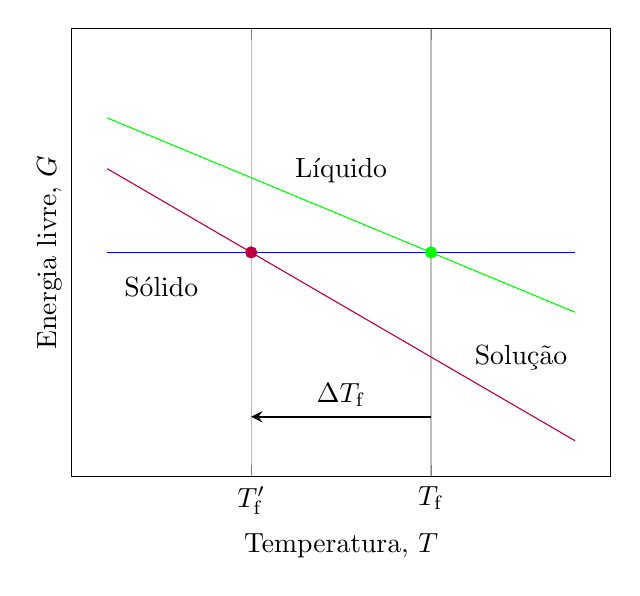
\begin{tikzpicture}
\begin{axis}
    [
        grid = major,
        ylabel = {Energia livre, $G$},
        xlabel = {Temperatura, $T$},
        domain = 0.2:2.8,
        xmin = 0, xmax = 3,
        ymin = -20, ymax = 10,
        xtick= {1, 2}, 
        xticklabels={$T_\mathrm{f}^\prime$, $T_\mathrm{f}$},
        ytick=\empty,
    ]
    \addplot [ purple ]
        { 2-7*x };
    \node [anchor = south] at (axis cs:2.5, -13.5) 
        { Solução };

    \addplot [ green ]
        { 5-5*x };
    \node [anchor = south] at (axis cs:1.5, -1) 
        { Líquido };

    \addplot [ blue ]
        { -5 };
    \node [anchor = north] at (axis cs:0.5, -6) 
        { Sólido };

    \addplot [ mark=*, color=purple, only marks ] coordinates
        { (1, -5) };
    \addplot [ mark=*, color=green, only marks ] coordinates
        { (2, -5) };

    \draw [ draw=black, thick, -stealth ]
        (axis cs: 2, -16) -- node [above] {$\Delta T_\mathrm{f}$}
        (axis cs: 1, -16);
\end{axis}
\end{tikzpicture}
